\chapter{Challenges In Relative Pose Estimation}

The success of recovery of relative pose mainly depends on two factors: The
accuracy and correctness of image point correspondences and them not being in
a degenerate configuration, so that they provide enough information about the
scene.

This chapter will examine the preconditions and the feasibility of pose recovery
in realistic conditions. Several problematic cases will be identified and
described. Furthermore, an assessment of different feature detection algorithms
for the purpose of this work will be given.

\section{Degenerate Configurations}

Degenerate configurations are those in which the data on which the essential
matrix is estimated allows for more than one mathematically valid solution. Two
different cases can be observed.

\subsection{Structure degeneracy}

Structure degeneracy is a configuration of points in the observed scene which do
not provide enough information to wholly determine an essential matrix. The
projection matrix $P\in\mathbb{R}^{3\times3}$ with 
\begin{equation*}
   \mbf{x} = P\mbf{X}
\end{equation*}
has twelve elements but is a projective quantity, so all non-zero multiples of
$P$ are equivalent, wherefore it has only eleven degrees of freedom.  A
degenerate case is for instance when all points observed by the two cameras lie
on the same plane (or worse, a subspace of even lower dimension). The images of
a planar surface in two cameras as well as the planar surface itself and its
image are related by a homography \citep[see][ch. 13]{h&z2004}, which is a
mapping between planes and has eight degrees of freedom (being a $3\times3$
matrix and a projective element), meaning that three degrees of freedom are
undetermined \citep{torr1999}. A set of coplanar points alone thus does not provide
enough information to uniquely determine an epipolar geometry.

However, not all algorithms are susceptible to this problem. While the 8-point
algorithm alone cannot deal with this case, the five-point algorithm can and is
generally more robust \citep{li2006}. While there are other approaches to work
around such issues (e.g. an algorithm developed by \citet{chum2005} or
\citet{decker2008}), in practice, a five-point algorithm in a RANSAC scheme
works well and needs fewer iterations than an 8-point approach \citep{li2006}.

\subsection{Motion Degeneracy}

A second type of degeneracy occurs when the camera motion between two images has
fewer degrees of freedom than the model to be estimated---the essential matrix.
If the camera only translates or only rotates between images, the motion has
maximally three degrees of freedom. As \citet{decker2008} point out, an
essential matrix estimated under such conditions could be consistent with all
correct point matches, but also with some false ones due to the mismatch in
degrees of freedom between data and model. In schemes like RANSAC, such an
estimate will have a large consensus set---all inliers \emph{plus}
outliers---and so may lead to the termination of the algorithm, despite being
inaccurate.

It is unlikely in rephotography that the observed scene will be completely
planar, or that the user will move from the first frame in a motion which is
pure rotation or translation, these degeneracies can be labelled edge cases and
are not specifically handled in the application.

\section{Finding Correspondences}

There is a variety of automatic feature detection algorithms which differ in
repeatability, robustness to noise, speed and invariance with respect to image
characteristics such as scale, brightness, or rotation. 
Generally, a feature detector identifies potentially salient points in an image
and computes a descriptor for these points in a way that the same point under
different conditions will yield an ideally identical descriptor. When points of
interest---usually called \emph{keypoints}---are available in multiple images,
their descriptors can be compared and the best match according to some metric
can be selected for each keypoint. The matches found can then be used as
corresponding points for relative pose estimation.

Classical state-of-the-art detectors include e.g. \emph{Scale-invariant feature
transform} \citep{lowe1999}, \emph{Speeded-up robust features}
\citep{bay2006} which both compute real-valued descriptors. A natural criterion
for selecting the best matching keypoint for a given keypoint is the $L_2$-norm
of the difference of their descriptors, which is a relatively expensive
operation. While e.g. SURF improves performance over the computationally
demanding SIFT detector, the speed of matching can still present a bottleneck in
time-critical contexts. The proliferation of mobile devices with more economic
hardware increased the demand for faster detection and matching of features and
many solutions have been proposed. On the one hand, efforts have been made at
faster feature detection algorithms in general (such as SURF or FAST
\citep{rosten2005}), but most promising are those which compute binary instead
of real-valued descriptors. The matching of $n$ features between images is an
$\mathcal{O}(n^2)$ operation when done with brute force, thus often placing a
limit on the computational efficiency of the whole process. On real hardware,
floating point operations are generally less efficient when compared to integer
or binary arithmetic. While for real-valued descriptors $d_1,~d_2$ with size $n$,
an $L_2$-norm 
\begin{equation*}
   \sqrt{\sum_{i=1}^n (d_1^i - d_2^i)^2}
\end{equation*}
must be evaluated,
binary strings can be compared with the Hamming distance 
\begin{equation*}
   \sum_{i=1}^n d_1^i \otimes d_2^i   
\end{equation*}
which is much faster. These descriptors include but are not limited to BRIEF
\citep[Binary Robust Independent Elementary Features]{calonder2010}, ORB
\citep[Oriented BRIEF]{rublee2011} and FREAK \citep[Fast Retina
Keypoint]{ortiz2012}. While some invariances are sacrificed in favour of
performance (such as rotation invariance of BRIEF, corrected by ORB), they are
claimed to match the repeatability of SIFT and others for many use cases while
being much faster to compute and compare. Another recent development by
\citet{alcantarilla2013} are AKAZE features, building on and accelerating the
previously proposed KAZE detector \citep{alcantarilla2012}, also using binary
strings to describe feature points. This detector has been chosen for this work
as it offers significant speed improvements over SIFT or SURF while sacrificing
no quality in the tested scenarios (see \autoref{ch:evaluation}).

\subsection{SIFT \& AKAZE}

The SIFT detector attempts to find keypoints by convolving an input image with
gaussian kernels of successively larger variance, thus building a stack of image
\emph{scales}. This process is repeated for several \emph{octaves}, each starting
from a downsampled version of one of the blurred images from the previous scale
octave. The resulting pyramid is termed \emph{scale space}.  From these gaussian
images, difference-of-gaussians are computed by subtracting neighbours in scale
space. These difference images approximate an application of the Laplacian of
Gaussian (a Laplacian filter with prior smoothing to remove noise) which computes
the second spatial derivatives of the image and whose extremes are locations of
rapid intensity change like edges or corners. Within this scale space, extrema
are found which are such pixels in the DOG images whose absolute values are
maximal or minimal in comparison with their twenty-six neighbours in scale
space. This search is conducted in all DOG images for all octaves which
contributes to the scale invariance. After locating the keypoint with subpixel
accuracy in the image, keypoints are discarded if their absolute DOG value is
below some threshold as those are unstable and unlikely to be found under
differenc conditions. Furthermore, the Hessian of the
image (the matrix of second-order partial derivatives of the image intensity
function) is computed to filter out keypoints on edges as they are not accurately
localised and thus likewise unstable. Descriptors are computed by assigning a
primary orientation after analysing the intensity gradients in the region around the
keypoint and binning them into histograms. A keypoint's coordinate system is
rotated according to this primary orientation, thus achieving rotation
invariance. The resulting descriptor has 128 elements which will occupy at least
as many bytes.

In contrast to SIFT, where the scale space construction is linear since
convolution is linear, the scale space in AKAZE is nonlinear. Gaussian blurring
(a form of isotropic diffusion) at successively higher scale smooths not only
noise, but also true object boundaries which decreases the accuracy of
localising keypoints. A nonlinear scale space blurs the image in a way that
respects the local image structure and thus preserves object boundaries while
smoothing out noise. A visualisation of the difference is shown in
\autoref{fig:lin_vs_nonlin_diffusion}. The diffusion is large in homogeneous
areas and small in areas of significant intensity change.  A nonlinear scale
space is built for AKAZE by means of fast explicit diffusion
\citep{grewenig2010} and the diffusivity is adapted by considering the magnitude
of the image gradient at a given point---meaning that it will be smaller for
areas of strong change and larger for others. As in SIFT, the scale space
consists of several octaves, each downsampled by two with respect to the
previous octave. The Hessian matrix determinant is used to identify possible
keypoints (in SIFT, this is used to filter out bad candidates),  but the
candidate must be extremal compared to other keypoint candidates in its
neighbourhood instead of neighbouring pixels. The window searched depends on the
scale at which the keypoint is located (the window is larger at higher scales
with more blur).

\begin{figure}[h]
   {\centering      
      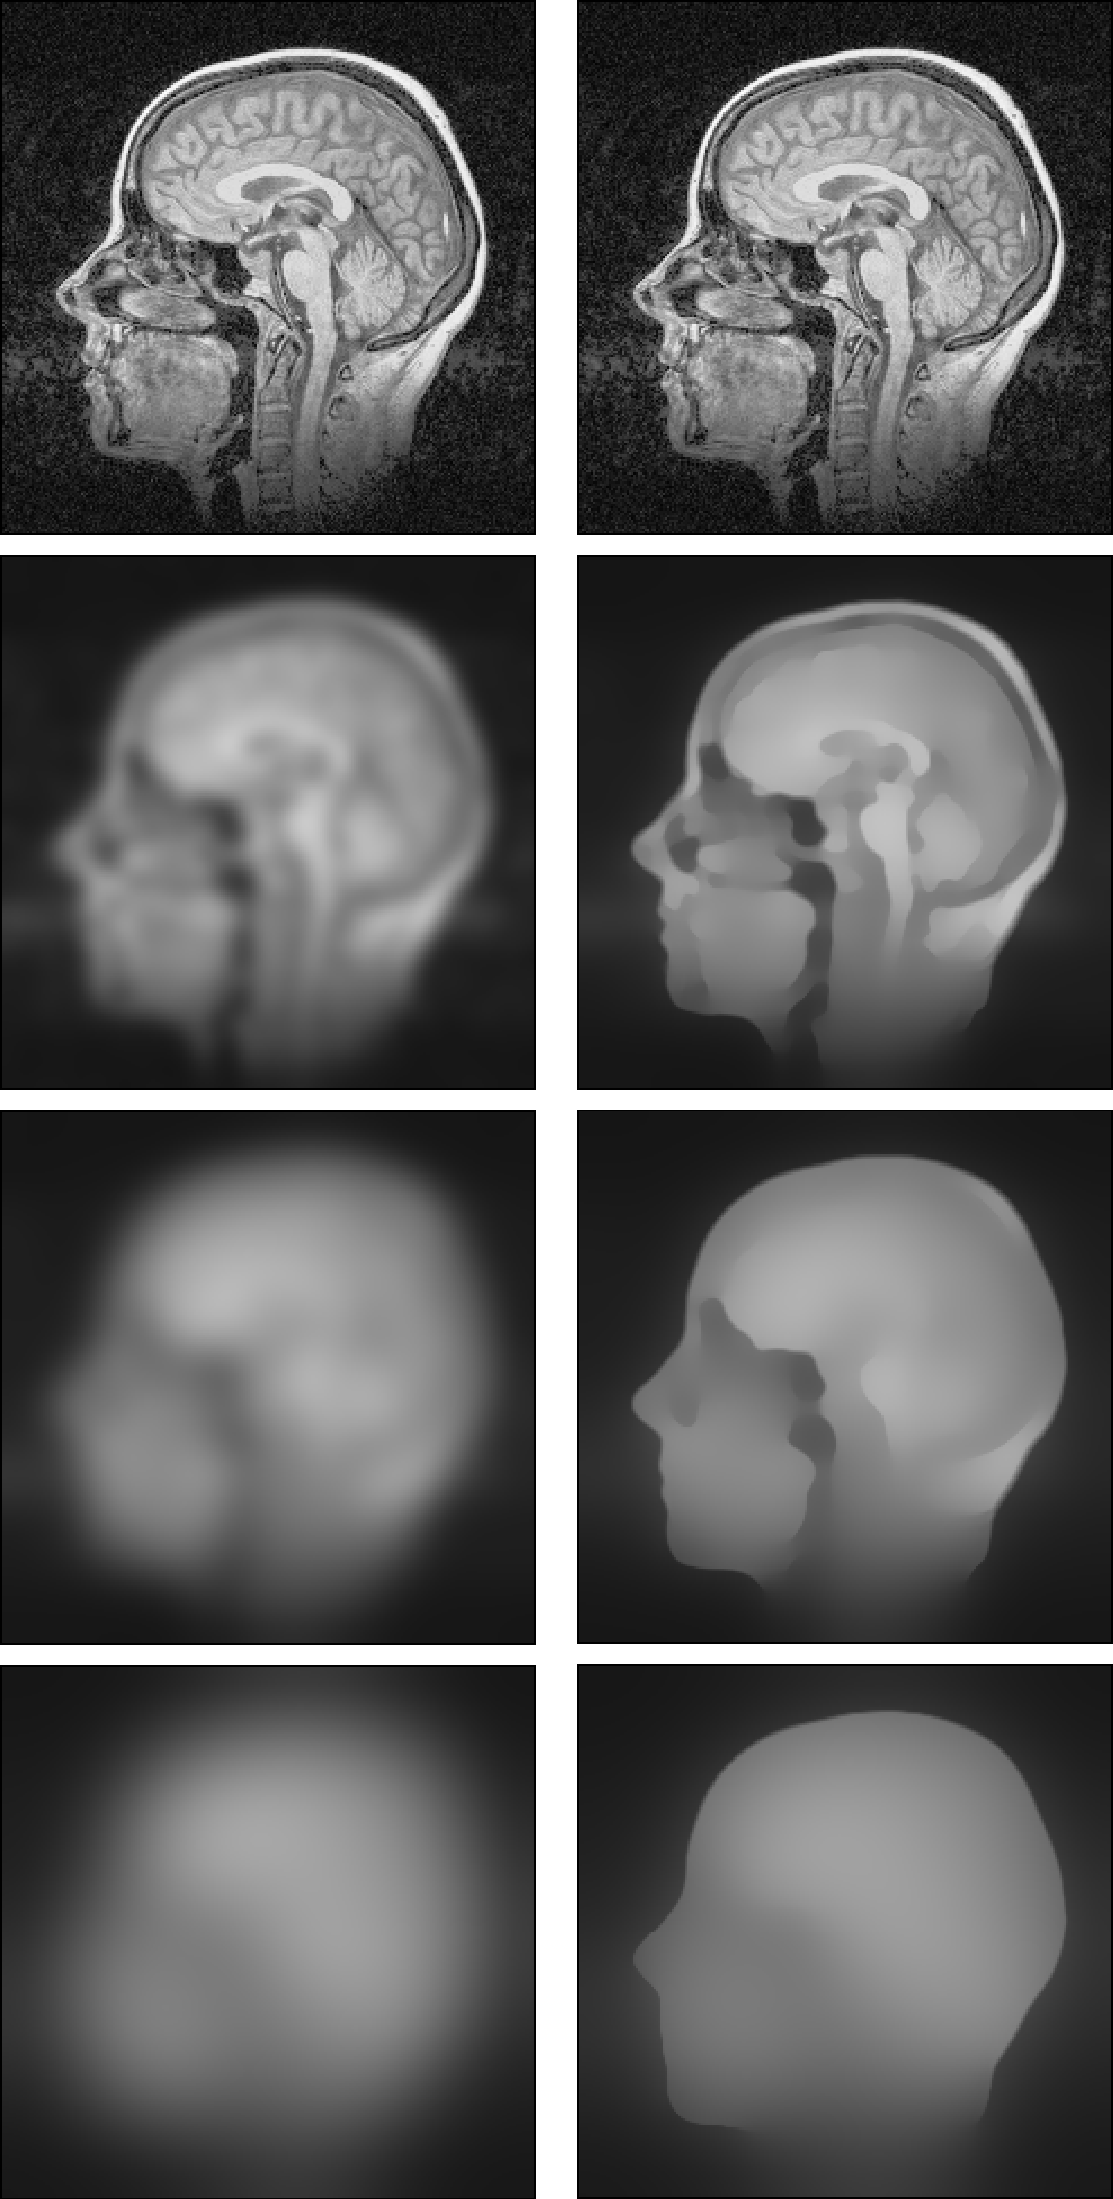
\includegraphics[width=.5\textwidth]{gfx/lin_vs_nonlin_diffusion2.png}
      \caption[Linear vs. nonlinear diffusion]{Image from \citep[p.120,121]{weickert1998}. Linear diffusion on the left,
   anisotropic nonlinear diffusion on the right.}
   \label{fig:lin_vs_nonlin_diffusion}}
\end{figure}

The AKAZE descriptor is obtained from dividing the image region around a
keypoint into a grid and then performing binary tests between all such grid
cells $i,~j$ which test whether $f(i) > f(j)$ for some function $f$ which
encapsulates some information of the cell \citep{yang2012}. To achieve rotation
invariance, this grid is rotated according to the dominant orientation computed
by considering the image derivatives---already computed for the detection---in
the neighbourhood \citep{alcantarilla2012}. The results of these binary tests are
assembled into a binary vector. Its size can be adjusted by making the grid
coarser or finer.

\section{Sorry, no title available}

\tikzexternaldisable
\begin{tikzpicture}[
      every node/.append style={font=\small,text width=1.5cm,text centered},
   boxnode/.style={outer sep=0,inner
sep=4pt,fill=RoyalBlue,text=white,draw=gray,shape=rectangle,rounded
corners=5pt,minimum height=1.3cm}]
\tikzset{>=latex}
\node[boxnode] (ref) {Reference photo};
\node[boxnode,right=of ref] (first frame) {First frame};
\node[boxnode,right=of first frame] (second frame) {Second frame};
\node[draw] (t first ref) at ($(ref) !.5! (first frame) + (0,-3cm)$) {$T_{first,ref}$};

\node[inner sep=0,shape=circle,draw] (triangulation) at ($(first frame) !.5! (second frame) +
(0,-3cm)$) {Triangu-lation};

\coordinate (c) at ($(t first ref.north) + (0,1em)$);
\draw[->] (ref.south) |- (c) -- (t first ref);
\draw[->] (first frame.south) |- (c) -- (t first ref);
\draw (first frame) -- coordinate[midway] (c) (second frame);
\draw[->] (c) -- (triangulation);
\draw[->] (triangulation) -- (t first ref);

\end{tikzpicture}
\tikzexternalenable

